% NeuroEvoScientist — ARR October 2026 submission (anonymous, double-blind)
% Built from the locked manuscript (paper/manuscript_v3.md, commit-anchored).
% No scientific divergence from the locked Markdown; LaTeX is formatting only.

\documentclass[11pt]{article}
\usepackage[review]{acl}
\usepackage{times}
\usepackage{graphicx}
\usepackage{booktabs}
\usepackage{latexsym}
\usepackage{multirow}
\usepackage{array}
\usepackage{amsmath}

\title{Task-Conditioned Cognitive Architecture Co-Design for LLM Agents:\\
A Controlled Study of Generalization, Cost, and Failure Modes}

\author{Anonymous ARR submission}
\date{}

\begin{document}
\maketitle

\begin{abstract}
LLM agents are usually deployed with a fixed, manually designed cognitive
architecture. We ask whether per-task co-design of an agent's reasoning
strategy, episodic memory/exemplar policy, and context allocation---above a
frozen backbone---materially changes capability--cost behavior, and whether
task-conditioned search generalizes. We present NeuroEvoScientist, a
controlled study over a structured family of agent configurations with
leakage-safe calibration splits, raw multi-objective logging, task-aware
phenotype canonicalization, pre-registered holdout evaluation, and paired
item-level statistics across two frozen backbones (Qwen2.5-1.5B and 7B).
On untouched GSM8K holdout, a searched configuration outperforms the
strongest fixed baseline by +29.0 percentage points at 1.5B and +16.7
points at 7B (McNemar $p<0.001$), while controlled same-genome ablation
shows memory contributions that grow with backbone scale. Search-side
architecture preferences differ clearly and stably by task---a long-context
scientific-QA task shifts the optimum to retrieval-based memory, as
pre-registered---yet dev-selected task-specific architectures do not
universally generalize: on PubMedQA and QASPER holdout they are beaten by
the configuration selected for GSM8K. A QASPER configuration that works at
1.5B collapses at 7B; our diagnostic shows this is an
answer-format/extraction interaction, not a capability failure.
Equal-budget evolutionary search does not beat random search in this
compact space, and a real trainable Mamba-2 substrate is not selected as
beneficial; we report both as audit findings. The work contributes a
leakage-safe, falsifiable protocol for agent architecture co-design and a
careful map of where task-conditioned specialization does---and does
not---generalize.
\end{abstract}

\section{Introduction}

LLM agents are typically assembled by hand: a reasoning pattern, a memory
mechanism, and a context budget are chosen once and reused across tasks. Yet
different tasks place different demands on each component---multi-step
arithmetic rewards explicit reasoning steps, biomedical judgment rewards
calibrated abstention, and long-document question answering rewards context
allocation and evidence retrieval. We ask two questions. First, do these
cognitive architecture choices materially change an agent's capability--cost
behavior when the underlying language model is kept frozen? Second, can
automatic, task-conditioned search over such choices find configurations
that remain superior on data untouched by the search itself?

We answer both with NeuroEvoScientist, a controlled co-design framework in
which an agent configuration is a structured genome over reasoning strategy,
episodic memory policy, and context policy, evolved with multi-objective
selection and evaluated under a leakage-safe, pre-registered protocol. Our
study deliberately audits its own search procedure: we enumerate the compact
search space exhaustively to obtain a ground-truth landscape, we compare
evolutionary search to equal-budget random search at budgets below full
coverage, and we hold out benchmark items that the search never sees.

Our findings are deliberately two-sided. On the positive side, architecture
choices matter enormously: searched configurations beat the strongest fixed
baseline by up to +29 percentage points on held-out GSM8K, task-specific
gene distributions are stable across seeds, and a pre-registered
prediction---that a long-context task shifts the optimum toward retrieval
memory---is confirmed. On the negative side, dev-selected task-specific
architectures do not universally generalize; equal-budget random search
matches evolutionary search in our compact space; and a real Mamba-2
substrate, though correctly implemented and trainable, is not selected as
beneficial. We report these negative results as part of the contribution.

\section{Related Work}

\paragraph{Agent architectures and workflow optimization.}
LLM agents commonly chain reasoning and acting through manually designed
scaffolds~\citep{yao2023react,schick2023toolformer} or self-reflection
loops~\citep{shinn2023reflexion}; DSPy compiles declarative LLM calls into
optimizable pipelines~\citep{khattab2023dspy}. These frameworks optimize
prompts or workflow structure; we instead co-design an agent's cognitive
configuration---reasoning strategy, episodic memory policy, and context
allocation---under explicit capability--cost objectives with a frozen
backbone.

\paragraph{Automated agent search.}
Most closely related are automated agent-design frameworks: ADAS searches
over agent programs expressed in code~\citep{hu2024adas}, and AgentSquare
searches a modular design space of planning, reasoning, tool-use, and memory
modules~\citep{shang2025agentsquare}. Both optimize for performance alone.
We differ by (i) searching per-task cognitive configurations with real
memory substrates rather than workflow topology; (ii) evaluating under
multiple raw objectives instead of a single score; and (iii) pre-registered
held-out auditing with paired statistics, reporting where specialization
does and does not generalize.

\paragraph{Prompt and reasoning strategy optimization.}
Chain-of-thought prompting materially affects reasoning
accuracy~\citep{wei2022cot}, and EvoPrompt evolves prompt
text~\citep{guo2024evoprompt}. We treat the reasoning strategy as one gene
jointly searched with memory and context policy.

\paragraph{Episodic and retrieval memory.}
Retrieval-augmented generation grounds LLMs in external
evidence~\citep{lewis2020rag}. Our memory policies manage a
calibration-only experience bank, and we quantify when episodic memory
helps, hurts, or is neutral across tasks and backbones.

\paragraph{Evolutionary computation and NAS.}
Neural architecture search is surveyed by \citet{elsken2019nas};
regularized evolution is a strong NAS baseline~\citep{real2019ameoba}, and
multi-objective selection follows NSGA-II-style non-dominated sorting with
crowding distance~\citep{deb2002nsga2}. Bayesian optimization is the
standard sample-efficiency reference~\citep{shahriari2016bayesopt}. Unlike
NAS over backbone weights, our search operates above a frozen LLM, and we
audit the search procedure against equal-budget random search on a fully
enumerated landscape.

\paragraph{Automated discovery and memory models.}
AlphaEvolve evolves programs through LLM proposals and
evaluators~\citep{alphaevolve2025}; we share the evolutionary loop but
change the object of evolution. Mamba and Mamba-2 provide the selective
state-space models from which our real trainable memory substrate is
built~\citep{gu2023mamba,dao2024mamba2}.

\paragraph{Benchmarks and backbones.}
We evaluate on GSM8K~\citep{cobbe2021gsm8k}, PubMedQA~\citep{jin2019pubmedqa},
and QASPER in its LongBench form~\citep{dasigi2021qasper,bai2023longbench},
using frozen Qwen2.5-Instruct backbones~\citep{yang2024qwen25}. We claim no
priority over any of these works; our contribution is a controlled,
leakage-safe, multi-objective audit of task-conditioned co-design, including
its failure modes. Parameter-efficient adapters such as
LoRA~\citep{hu2021lora} are related as adapter technology only; no LoRA gene
is searched or claimed in this paper.

\section{Problem Formulation}

An agent configuration is a genome over three gene families: memory policy,
reasoning strategy, and context policy. Given a task and a frozen backbone,
we seek configurations that occupy favorable positions on the
capability--cost Pareto frontier---not a single scalar optimum. Task
conditioning means the preferred configuration may differ per task; the
scientific question is whether search-side preferences correspond to
generalizable holdout advantages or merely to search-split overfitting.

\section{Method}

\subsection{Two protocol layers}

\paragraph{Compact audit layer.} A flat genome over memory
$\{\text{recency}, \text{retrieval}, \text{mamba2}, \text{hybrid}\}$,
reasoning $\{\text{direct}, \text{cot}, \text{verify}, \text{planner}\}$,
and context policy $\{\text{full}, \text{truncated}, \text{answer\_only}\}$
defines 48 configurations. We evaluate all of them per benchmark to obtain
an exhaustive landscape with raw objectives---capability, efficiency,
prompt-token cost, latency, and adaptation cost---used as an analysis oracle
for the search-efficiency audit.

\paragraph{Structured co-design layer.} The final search space refines each
gene with conditional sub-genes: memory recall width and similarity metric
(hashed bag-of-words cosine; explicitly not a learned dense retriever),
Mamba-2 state size, hybrid mixing fraction, reasoning depth and verifier
passes, exemplar word budget and count, input-context word budget for
long-document tasks, and a per-candidate substrate-adaptation budget.
Normalization removes semantically inactive sub-genes before hashing, so
duplicate phenotypes are never double-counted; task-aware canonicalization
additionally drops the input-context budget outside long-context tasks.

\subsection{Genes are real mechanisms}

All memory banks are built exclusively from calibration splits; test items
never enter the bank. \texttt{recency} returns the most recent $k$ entries;
\texttt{retrieval} returns similarity top-$k$; \texttt{mamba2} runs a real,
trainable Mamba-2 substrate over the bank as an ordered sequence and scores
candidates against the resulting order-dependent state; \texttt{hybrid}
mixes retrieval with the most recent entry. Reasoning genes are distinct
instruction templates; context genes change real exemplar verbosity and
document allocation. Candidates carrying the trainable substrate receive a
fixed adaptation budget (48 calibration samples, 30 AdamW steps, fixed
learning rate and seed) with the backbone frozen; substrate weights can be
inherited from parents as an appendix mechanism evaluated separately.

\subsection{Operators}

Mutations are local (neighboring values for ordered sub-genes), crossover
swaps semantic blocks and normalizes, and selection is NSGA-II-style
non-dominated sorting with crowding-distance diversity over raw objectives;
scalar fitness is used only for logging.

\section{Experimental Setup}

\subsection{Benchmarks and splits}

\begin{table}[h]
\centering\small
\begin{tabular}{@{}llll@{}}
\toprule
Benchmark & dev/search & holdout & calibration \\
\midrule
GSM8K & test[0:100] & test[100:1319] & train split \\
PubMedQA & samples[0:100] & samples[100:500] & samples[500:1000] \\
QASPER & items[0:50] & items[50:150] & items[150:200] \\
\bottomrule
\end{tabular}
\caption{Leakage-safe splits. Pairwise disjointness is enforced by unit
tests; selection locks were committed before any holdout inference.}
\label{tab:splits}
\end{table}

\subsection{Backbones and decoding}

Qwen2.5-1.5B-Instruct for search and selection; Qwen2.5-7B-Instruct for
transfer only (no re-search). Greedy decoding, 256 max new tokens, batch 32,
FP16. Exact model revisions and dataset acquisition details are in the
reproducibility statement (Section~\ref{sec:repro}).

\subsection{Audit protocols}

The compact-space audit compares online evolutionary search and uniform
random search at evaluation budgets $\{12, 24, 36, 48\}$ across 20 search
seeds (best capability, Pareto hypervolume, regret, epsilon-Pareto hits,
evaluations-to-threshold, AUC). All key holdout comparisons are paired at
the item level: bootstrap 95\% CIs (10{,}000 resamples, fixed seed) and
exact McNemar tests.

\section{Main Results}

\subsection{R1: architecture choices matter materially}

\begin{table*}[t]
\centering\small
\begin{tabular}{@{}lcccccc@{}}
\toprule
 & \multicolumn{2}{c}{GSM8K} & \multicolumn{2}{c}{PubMedQA}
 & \multicolumn{2}{c}{QASPER (F1)} \\
\cmidrule(lr){2-3}\cmidrule(lr){4-5}\cmidrule(lr){6-7}
Config & 1.5B & 7B & 1.5B & 7B & 1.5B & 7B \\
\midrule
A\_gsm (searched) & \textbf{0.519} & \textbf{0.860} & 0.490 & 0.648 & 0.188 & 0.188 \\
A\_pubmed (searched) & 0.097 & 0.147 & 0.373 & 0.488 & 0.111 & 0.006$^\dagger$ \\
A\_qasper (searched) & 0.208 & 0.196 & 0.563 & 0.578 & 0.138 & 0.006$^\dagger$ \\
best fixed baseline & 0.229 & 0.693 & 0.598 & 0.603 & 0.176 & 0.015 \\
no\_memory (ablation) & 0.519 & 0.734 & 0.363 & 0.578 & \textbf{0.201} & \textbf{0.214} \\
\bottomrule
\end{tabular}
\caption{Holdout capability (accuracy; QASPER: LongBench-compatible
normalized QA F1 on extracted answer) for the three task-selected
configurations, strongest fixed baselines, and the Phase-20 no-memory reference (the A\_gsm genome with memory disabled). Controlled causal memory ablations are reported separately in Table~\ref{tab:ablation}.
$^\dagger$Marker-side extraction mismatch diagnosed in Section 7 (not a
capability collapse).}
\label{tab:main}
\end{table*}

On untouched GSM8K holdout, A\_gsm beats the strongest fixed baseline by
+29.0 percentage points at 1.5B and +16.7 at 7B (McNemar $p<0.001$). On
PubMedQA, searched configurations produce competitive capability--cost
tradeoffs but not universal capability superiority---a fixed retrieval
baseline remains ahead at 1.5B---and we report this asymmetry rather than
hiding it.

\subsection{R2: task-conditioned selection is stable and interpretable}

Across three search seeds, GSM8K converges to chain-of-thought with light
recency memory, PubMedQA converges bit-identically to no-memory direct
answering on all three seeds, and QASPER converges to retrieval-based memory
with many exemplars and a reduced document budget---matching our
pre-registered prediction that a long-context task shifts the optimum toward
retrieval (Figure~\ref{fig:genes}). A sensitivity audit after task-aware
phenotype canonicalization leaves these families unchanged.

\begin{figure}[t]
\centering
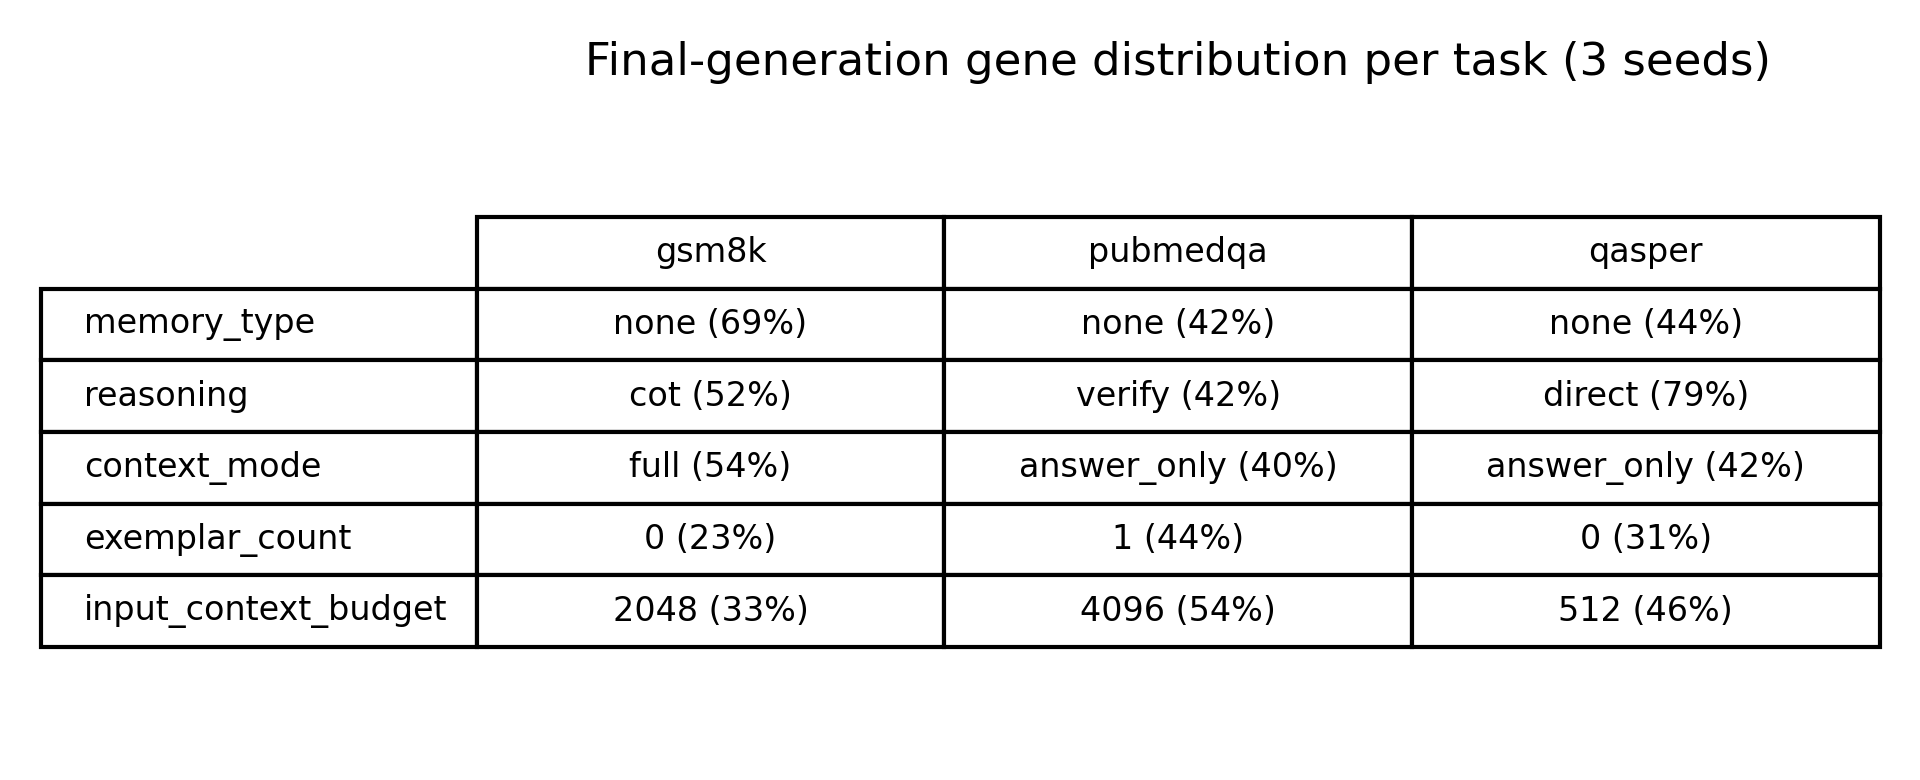
\includegraphics[width=\columnwidth]{figures/fig2_gene_distributions.png}
\caption{Final-generation gene distribution per task (mode and share over
three dev-search seeds).}
\label{fig:genes}
\end{figure}

\subsection{R3: dev-selected preferences do not universally generalize}

On GSM8K holdout, the own-task configuration dominates every alternative by
+31 to +71 points ($p<0.001$) in cross-task paired comparisons. On PubMedQA
and QASPER holdout, however, the task-selected configurations are beaten---
significantly---by the GSM8K-selected configuration
(Table~\ref{tab:transfer}). Search-side specialization is real, but
dev-slice preferences can overfit.

\begin{figure}[t]
\centering
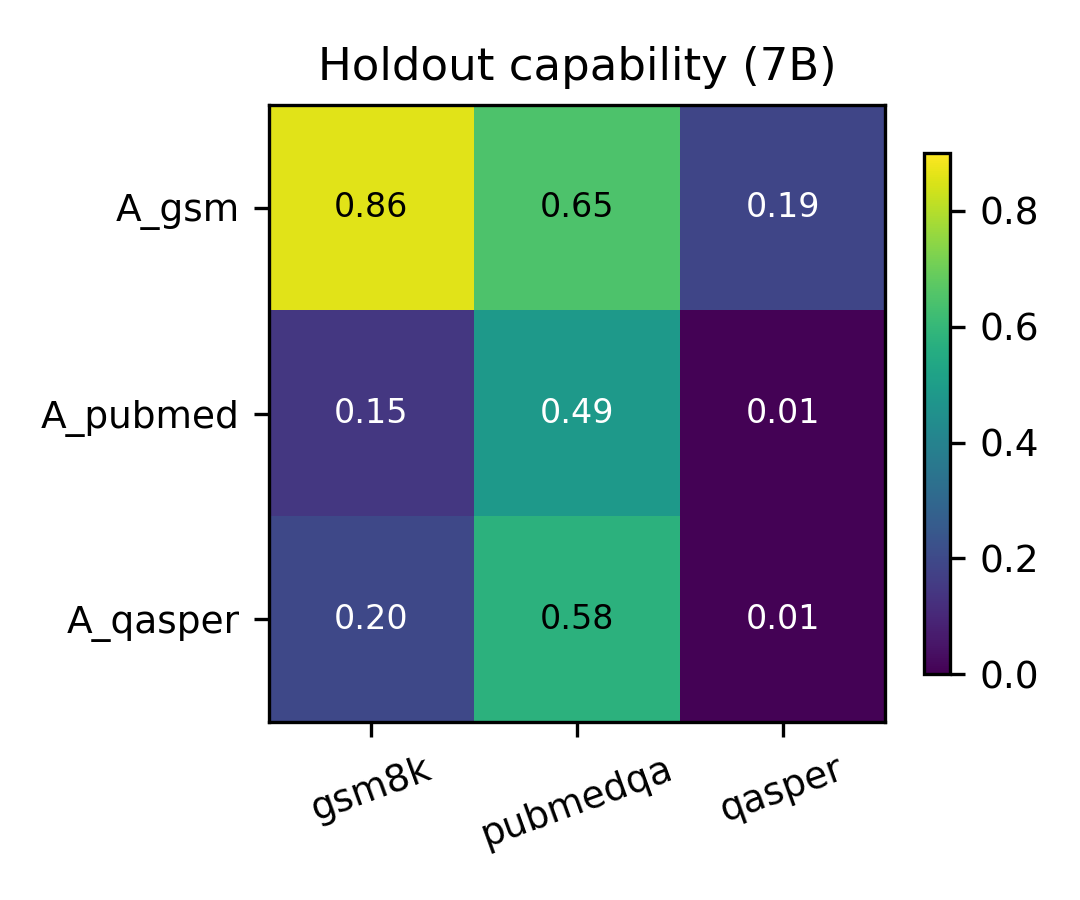
\includegraphics[width=\columnwidth]{figures/fig3_transfer_matrix_7b.png}
\caption{Holdout capability transfer matrix at 7B: rows are task-selected
configurations, columns are holdout benchmarks.}
\label{fig:transfer}
\end{figure}

\subsection{R4: memory contribution is controlled and scales with backbone}

Under same-genome ablation, removing episodic memory is neutral at 1.5B on
GSM8K but removes 12.6 points at 7B ($p<0.001$); on PubMedQA, enabling
memory on the frozen configuration adds +18.0 points at 1.5B; on QASPER the
effect is small (+1.5 points; Figure~\ref{fig:memabl}). Memory causality is
claimed only where the comparison is controlled.

\begin{figure}[t]
\centering
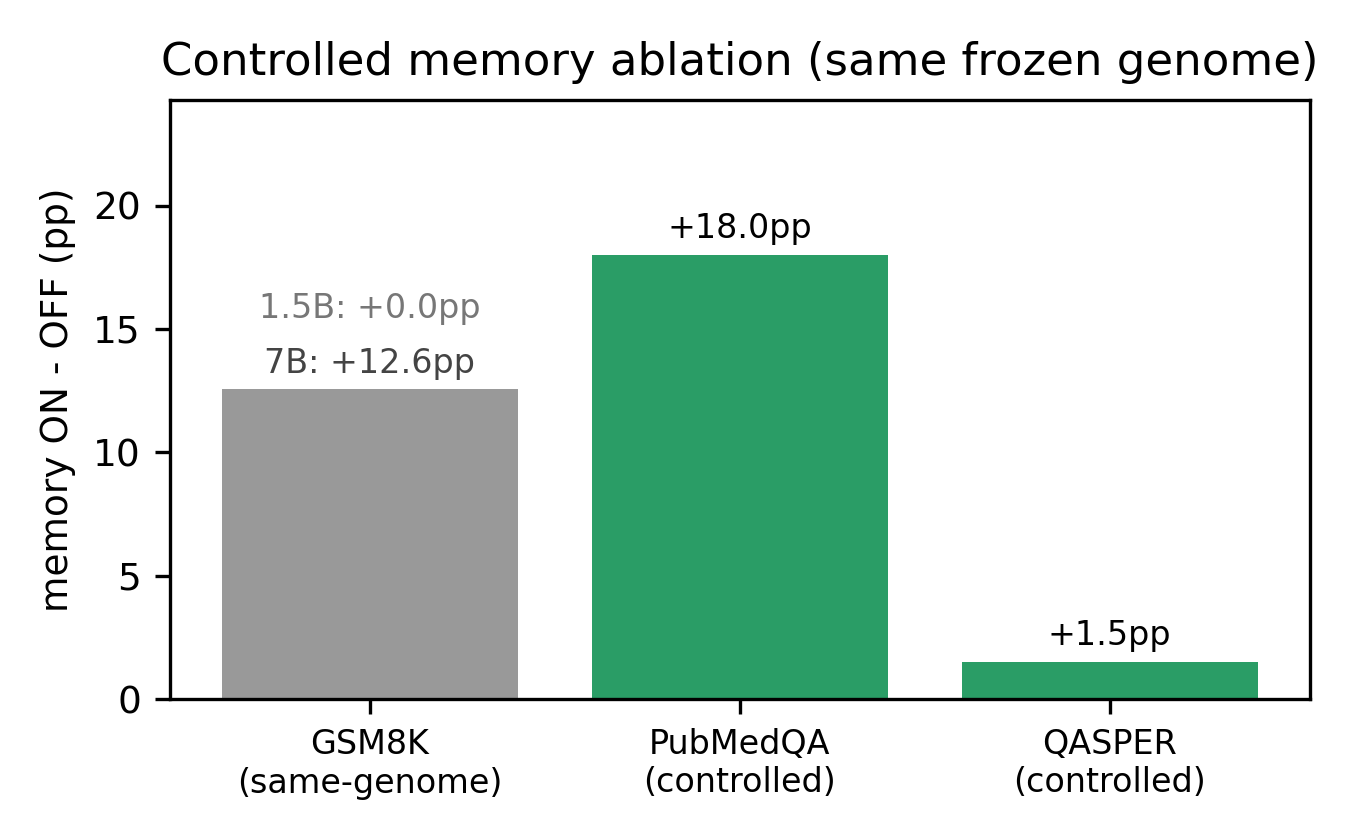
\includegraphics[width=\columnwidth]{figures/fig5_memory_ablation.png}
\caption{Controlled same-genome memory ablation across backbones.}
\label{fig:memabl}
\end{figure}

\begin{table}[t]
\centering\small
\begin{tabular}{@{}llcc@{}}
\toprule
Holdout task & Comparison (own vs cross) & 1.5B & 7B \\
\midrule
GSM8K & A\_gsm vs A\_pubmed & +42.2*** & +71.3*** \\
 & A\_gsm vs A\_qasper & +31.0*** & +66.4*** \\
\midrule
PubMedQA & A\_pubmed vs A\_gsm & $-$11.8*** & $-$16.0*** \\
 & A\_pubmed vs A\_qasper & $-$19.0*** & $-$9.0** \\
\midrule
QASPER & A\_qasper vs A\_gsm & $-$5.0* & $-$18.2*** \\
 & A\_qasper vs A\_pubmed & +2.7* & 0.0 \\
\bottomrule
\end{tabular}
\caption{Paired cross-task differences in holdout capability (percentage
points; bootstrap CI + exact McNemar; * $p{<}0.05$, ** $p{<}0.01$,
*** $p{<}0.001$). Positive favors the task-selected configuration.}
\label{tab:transfer}
\end{table}

\begin{table}[t]
\centering\small
\begin{tabular}{@{}llccc@{}}
\toprule
Task & Pair (same genome) & Backbone & ON & OFF \\
\midrule
GSM8K & A\_gsm $\pm$ memory & 1.5B & 0.519 & 0.519 \\
 & & 7B & \textbf{0.859} & 0.734 \\
PubMedQA & frozen recency $\pm$ memory & 1.5B & \textbf{0.553} & 0.373 \\
QASPER & A\_qasper $\pm$ memory & 1.5B & 0.125 & 0.111 \\
\bottomrule
\end{tabular}
\caption{Controlled same-genome memory ablation (capability; the only
causal memory comparisons in this paper).}
\label{tab:ablation}
\end{table}

\section{Generalization Audit and Failure Analysis}

\subsection{Search-efficiency audit}

The compact-space audit finds no search-efficiency advantage for
evolutionary search over equal-budget random search at any budget or
benchmark (differences below 0.01 in AUC and hypervolume across 20 seeds;
Figure~\ref{fig:landscape}). We therefore make no optimizer-superiority
claim; evolution is the architecture-generation mechanism, and our
contribution is the task-conditioned co-design evidence and the audit
protocol itself.

\begin{figure}[t]
\centering
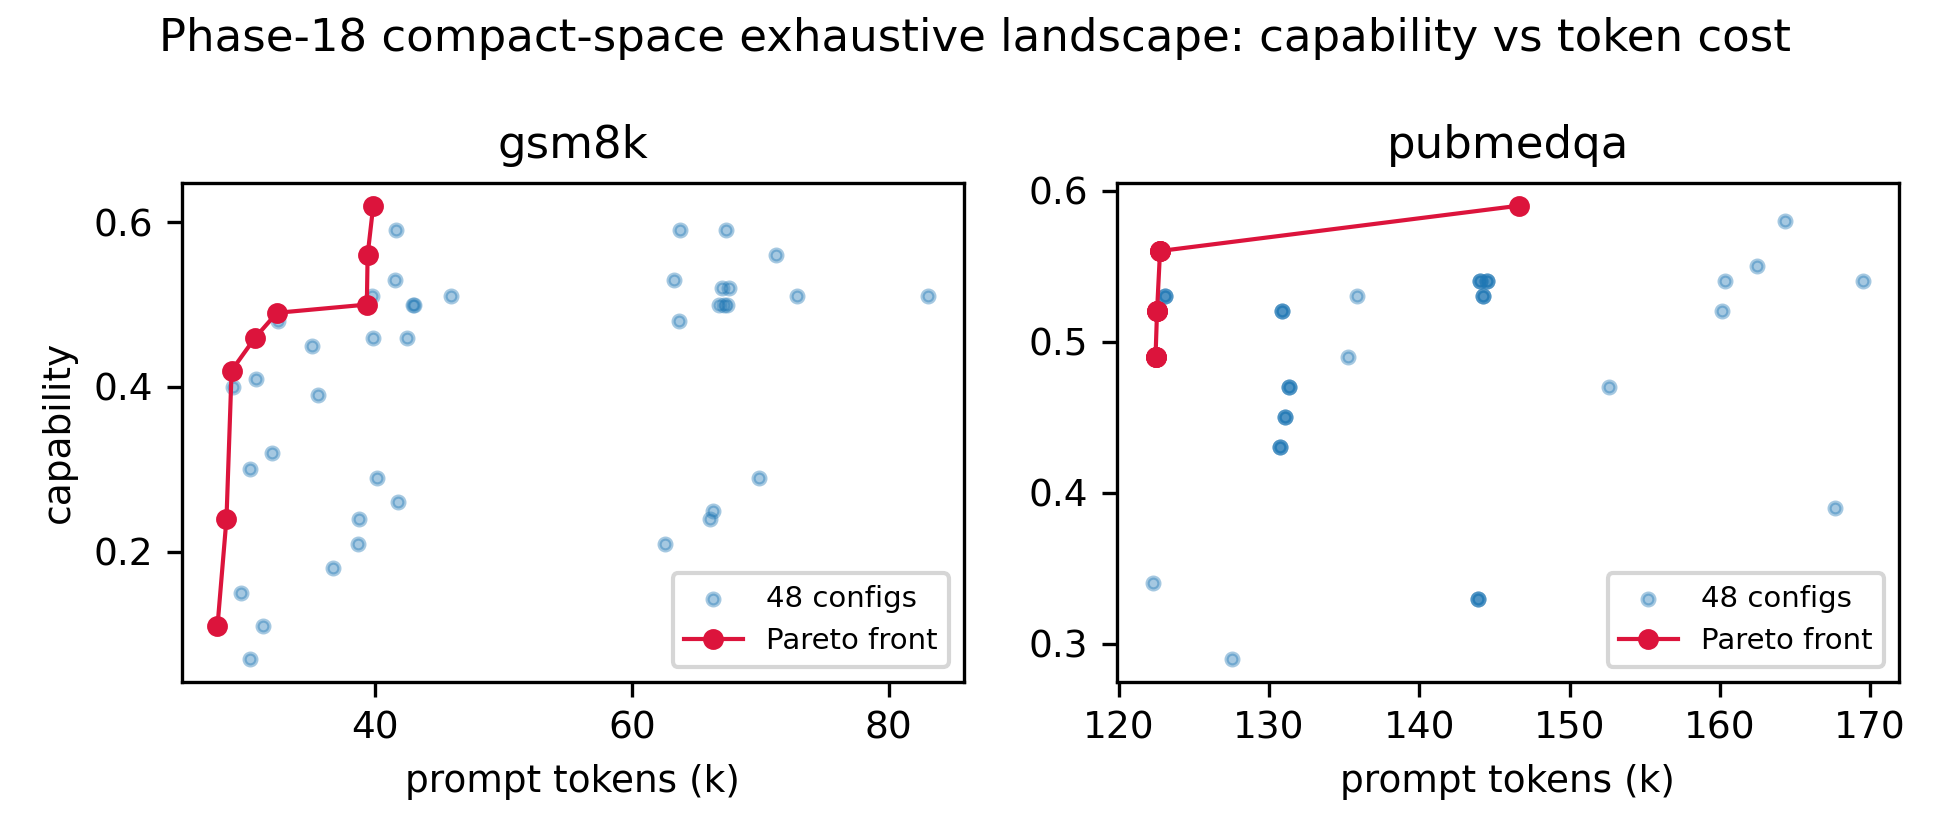
\includegraphics[width=\columnwidth]{figures/fig6_landscape_pareto.png}
\caption{Phase-18 compact-space exhaustive landscape (48 configurations per
benchmark): capability vs prompt-token cost, with the global Pareto front.}
\label{fig:landscape}
\end{figure}

\subsection{Negative results kept}

A real, trainable Mamba-2 substrate participates in the search but is not
selected as beneficial under our protocol; we keep this negative result.
Weight inheritance improves post-adaptation loss in all 20 paired cases but
yields no capability difference in any of them; it is reported as an
appendix mechanism.

\subsection{QASPER-7B failure diagnosed}

\begin{figure}[t]
\centering
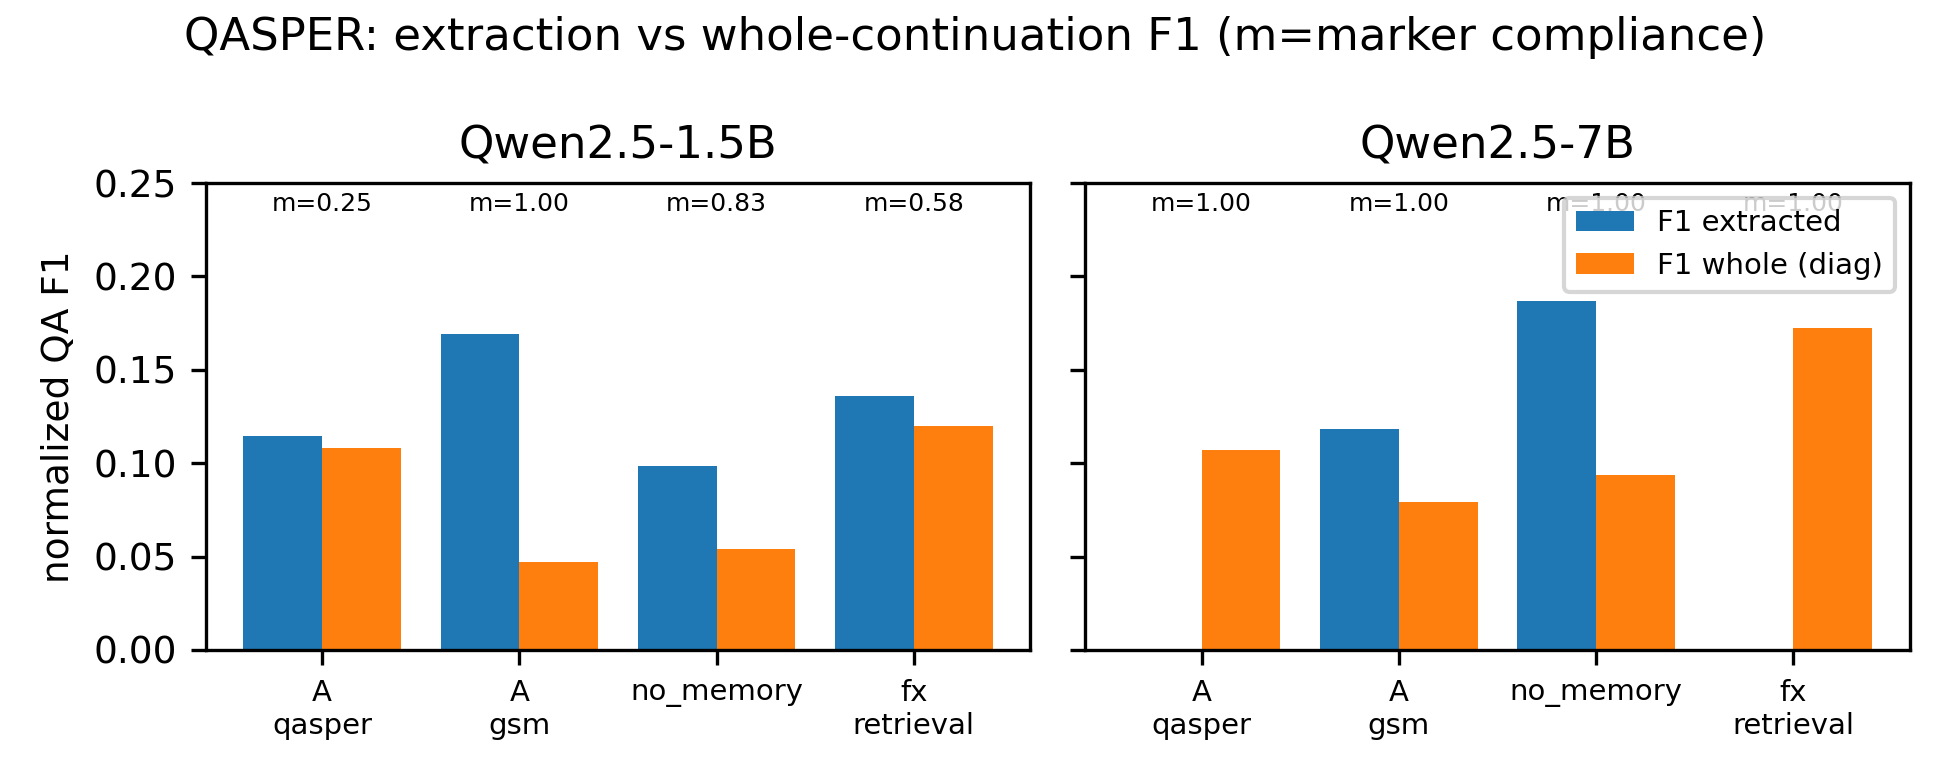
\includegraphics[width=\columnwidth]{figures/fig4_qasper_diag.png}
\caption{QASPER diagnostic: extracted-answer vs whole-continuation F1 at
1.5B and 7B, with marker compliance. The 7B ``collapse'' is an
answer-format/extraction interaction.}
\label{fig:diag}
\end{figure}

\begin{table}[t]
\centering\small
\begin{tabular}{@{}lcccc@{}}
\toprule
Config & Backbone & F1 (extr.) & F1 (whole) & marker \\
\midrule
A\_qasper & 7B & 0.000 & 0.107 & 1.00 \\
fixed\_retrieval & 7B & 0.000 & 0.172 & 1.00 \\
A\_gsm & 7B & 0.118 & 0.079 & 1.00 \\
no\_memory & 7B & 0.187 & 0.094 & 1.00 \\
\midrule
A\_qasper & 1.5B & 0.115 & 0.108 & 0.25 \\
A\_gsm & 1.5B & 0.169 & 0.047 & 1.00 \\
\bottomrule
\end{tabular}
\caption{QASPER diagnostic (12 fixed holdout items, frozen protocol):
marker compliance is perfect at 7B while extracted-answer F1 collapses,
diagnosing an answer-format/extraction interaction rather than a capability
failure.}
\label{tab:diag}
\end{table}

Several QASPER configurations appear to collapse at 7B (near-zero
extracted-answer F1). Our frozen diagnostic shows marker compliance is
perfect (100\%) while extracted-answer F1 is zero and whole-continuation F1
remains positive---the 7B backbone places its answer before or at the marker
instead of after it (Figure~\ref{fig:diag}). This is a
backbone--prompt/extraction interaction, not a capability failure.

\section{Mechanism Analysis}

Fourteen auditable case studies link genome choices to inference behavior:
successful and failed GSM8K items with recalled exemplars, PubMedQA
decisions, and paired QASPER 1.5B/7B failures with raw outputs and extracted
answers. These cases illustrate how exemplar content, context budget, and
answer-formatting instructions jointly shape outcomes.

\section{Limitations}

Our study uses a single model family (Qwen2.5 at 1.5B and 7B), a compact
audited space, prompt-level reasoning genes, and a single adaptation
protocol. PubMedQA's three-way ceiling limits capability separation, and
QASPER's answer extraction is marker-sensitive, which we diagnose rather
than hide. Cross-backbone latency is not compared without normalization.
Evolutionary superiority is not supported in our space; we do not claim it.
Small dev slices can overfit, as our own PubMedQA/QASPER results show.

\section{Conclusion}

Cognitive architecture choices materially change agent capability--cost
behavior. Automatic co-design exposes clear, stable, interpretable
task-conditioned preferences---and a rigorous held-out audit is what
distinguishes search-side specialization from generalizable advantage. We
release the full protocol, landscapes, per-item predictions, statistics, and
claim audit to make this kind of study falsifiable by construction.

\section{Reproducibility and Ethics Statement}
\label{sec:repro}

All experiments are frozen at the locked commits; exact model revisions,
dataset acquisition details, protocol parameters, cache semantics, and the
result-to-evidence map are documented in the anonymous reproducibility
package (supplementary material). The work uses public benchmarks and public
models, involves no human subjects, and reports negative results and failure
modes explicitly.

\bibliography{references}

\end{document}
